\lstinputlisting[language=bash,basicstyle=\small]{python_codes/fieldstone_111/keywords.ascii}

\begin{center}
Code at \url{https://github.com/cedrict/fieldstone/tree/master/python_codes/fieldstone_111}
\end{center}

\par\noindent\rule{\textwidth}{0.4pt}

%%%%%%%%%%%%%%%%%%%%%%%%%%%%%%%%%%%%%%%%%%%%%%%%%%%%%%%%%%%%%%%%%%%%%%%%%%%%%%%%%%%%%%%%%%%%%%%%%%%%

The derivations for this benchmark are found in Section~\ref{ss:elasticdisc}.
We here recall the fields for $n\ge 2$ and $k\ge 1$:
\begin{eqnarray}
\upnu_r          &=& \upnu_0 r^n \cos (k \theta)  \nn \\
\upnu_\theta     &=& \upnu_0 r^n \sin (k \theta)  \nn \\
\varepsilon_{rr} &=&   \upnu_0 n r^{n-1} \cos (k\theta) \nn\\
\varepsilon_{\theta\theta} &=&    \upnu_0 r^{n-1} (k+1) \cos (k\theta) \nn\\
\varepsilon_{r\theta} &=&  \cfrac{\upnu_0}{2}  r^{n-1}  (n-1-k)  \sin (k \theta)  \nn\\
\upnu_{rms}  &=& 2 \pi \upnu_0^2 \frac{R^{2n+2}}{2n+2} \nn\\
\sigma_{rr} 
&=& \lambda (\vec\nabla\cdot \vec\upnu) + 2 \mu \varepsilon_{rr} \nn\\
&=& \upnu_0  r^{n-1}  \cos (k\theta ) [\lambda (n+k+1)+2\mu n]  \nn\\
\sigma_{\theta\theta} 
&=& \lambda (\vec\nabla\cdot \vec\upnu) + 2 \mu \varepsilon_{\theta\theta}\nn  \nn\\
&=& \upnu_0  r^{n-1} \cos (k\theta ) [\lambda(n+k+1) + 2 \mu (k+1) ]  \nn\\
\sigma_{r\theta} 
&=& 2\mu \sigma_{r\theta} \nn\\
&=& \mu \upnu_0  r^{n-1}  (n-1-k)  \sin (k \theta) \nn 
\end{eqnarray}
Note that the $\upnu_{rms}$ is independent of $k$.

In what follows the disc has radius $R=1$. 
We set $\upnu_0$ and choose $\mu=1$, the Poisson ratio $\nu=0.25$ so that 
$\lambda=2\mu\nu/(1-2\nu)=1$.
The mesher is borrowed from \stone~58. The mesh consists of {\tt nLayers} concentric layers of elements.
We choose as 'diameter' of elements the value $h_r=R/nLayers$.
The code relies on first-order triangular elements ($P_1$).
The analytical displacement field is prescribed on the boundary.
Compared to \stone~58, this manufactured solution has the advantage that 
it provides displacement, strain and stress components everywhere in the disk:
these fields have a simple analytical expression and are finite.

The parameter $n$ influences the dependence in $r$ of the fields 
while the parameter $k$ influences the fields in the $\theta$ direction.

\newpage

\begin{center}
\includegraphics[width=5.7cm]{python_codes/fieldstone_111/results/u_k2}
\includegraphics[width=5.7cm]{python_codes/fieldstone_111/results/u_k3}
\includegraphics[width=5.7cm]{python_codes/fieldstone_111/results/u_k4}\\
\includegraphics[width=5.7cm]{python_codes/fieldstone_111/results/v_k2}
\includegraphics[width=5.7cm]{python_codes/fieldstone_111/results/v_k3}
\includegraphics[width=5.7cm]{python_codes/fieldstone_111/results/v_k4}\\
{\captionfont $u$ and $v$ fields for $n=2$. Left to right: $k=2,3,4$.}
\end{center}

\begin{center}
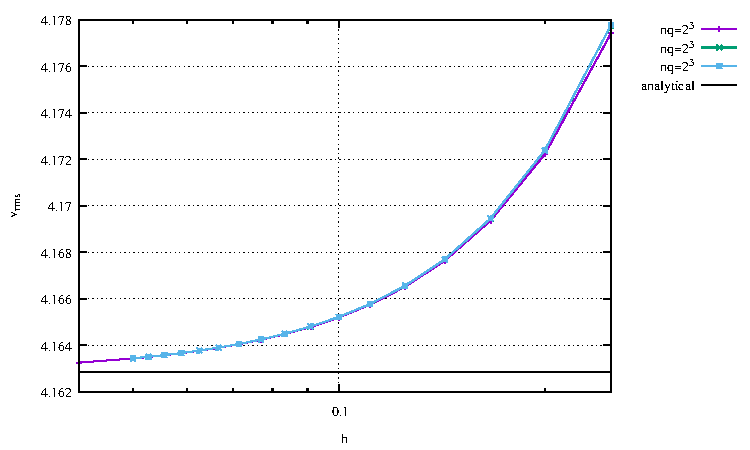
\includegraphics[width=7.4cm]{python_codes/fieldstone_111/results/vrms.pdf}
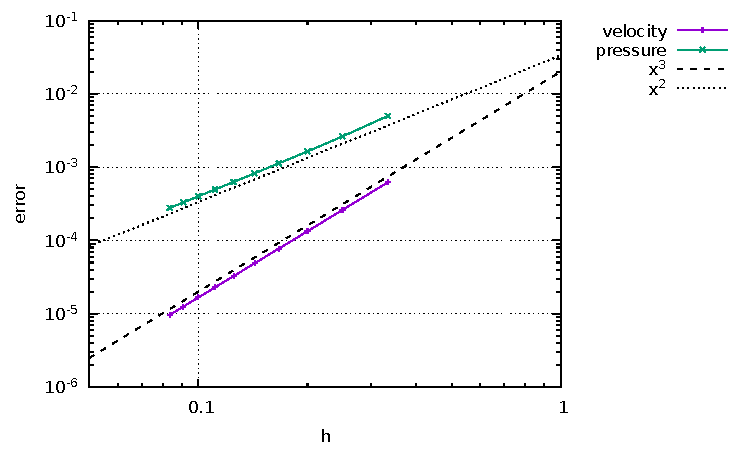
\includegraphics[width=7.4cm]{python_codes/fieldstone_111/results/errors.pdf}\\
{\captionfont Root mean square displacement and discretisation 
errors obtained with $n=2,3,4$ and $k=2,3,4$. Quadratic convergence 
is recovered as expected with linear elements.}
\end{center}

\newpage

\begin{center}
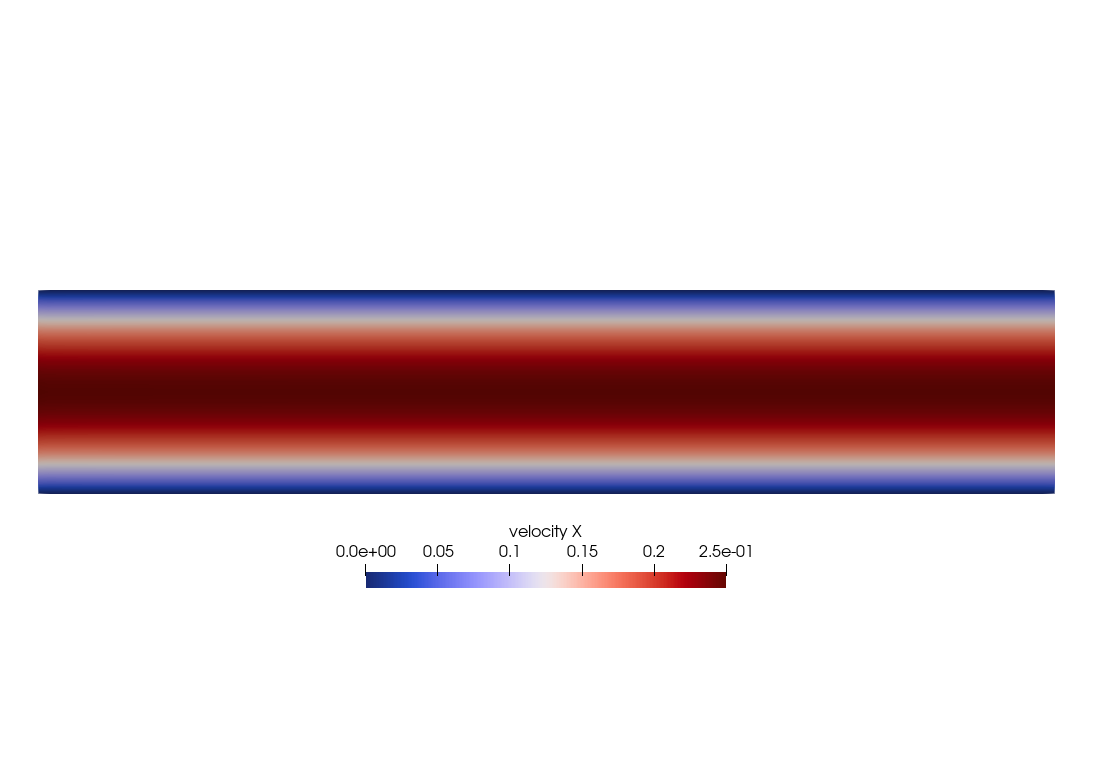
\includegraphics[width=7.2cm]{python_codes/fieldstone_111/results/n3_k5/u}
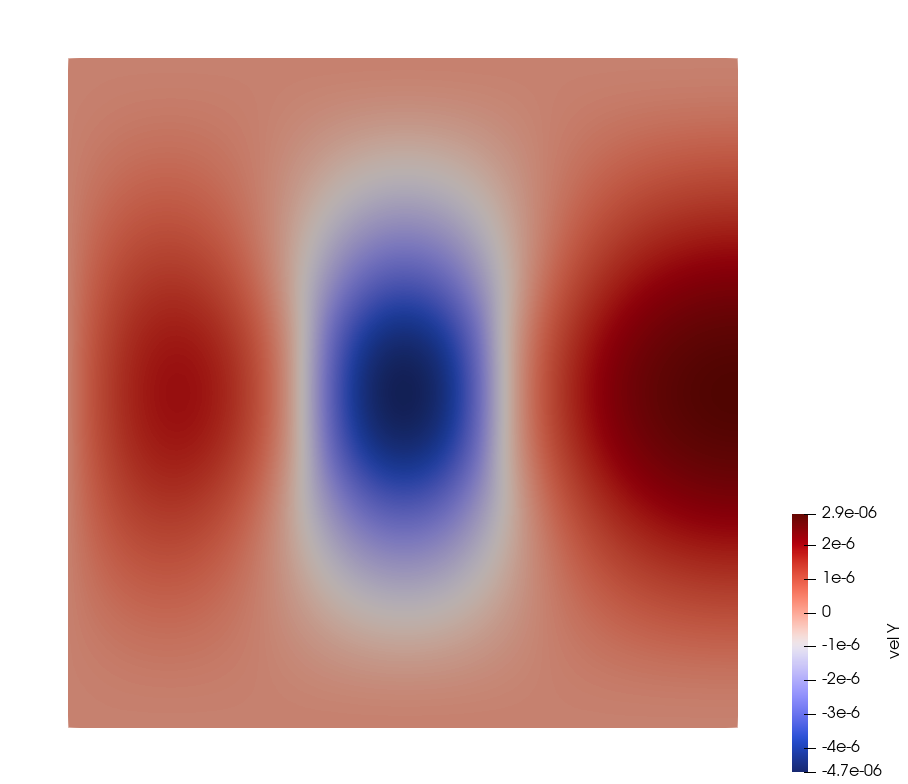
\includegraphics[width=7.2cm]{python_codes/fieldstone_111/results/n3_k5/v}\\
\includegraphics[width=5.7cm]{python_codes/fieldstone_111/results/n3_k5/e_xx}
\includegraphics[width=5.7cm]{python_codes/fieldstone_111/results/n3_k5/e_yy}
\includegraphics[width=5.7cm]{python_codes/fieldstone_111/results/n3_k5/e_xy}\\
\includegraphics[width=5.7cm]{python_codes/fieldstone_111/results/n3_k5/sigma_rr}
\includegraphics[width=5.7cm]{python_codes/fieldstone_111/results/n3_k5/sigma_tt}
\includegraphics[width=5.7cm]{python_codes/fieldstone_111/results/n3_k5/sigma_rt}\\
\includegraphics[width=5.7cm]{python_codes/fieldstone_111/results/n3_k5/e}
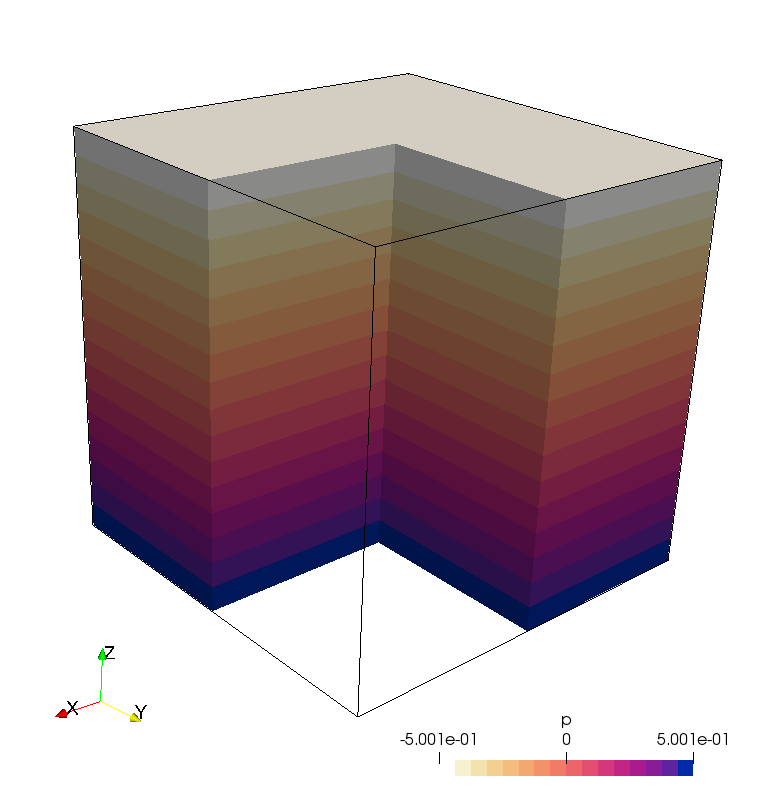
\includegraphics[width=5.7cm]{python_codes/fieldstone_111/results/n3_k5/press}
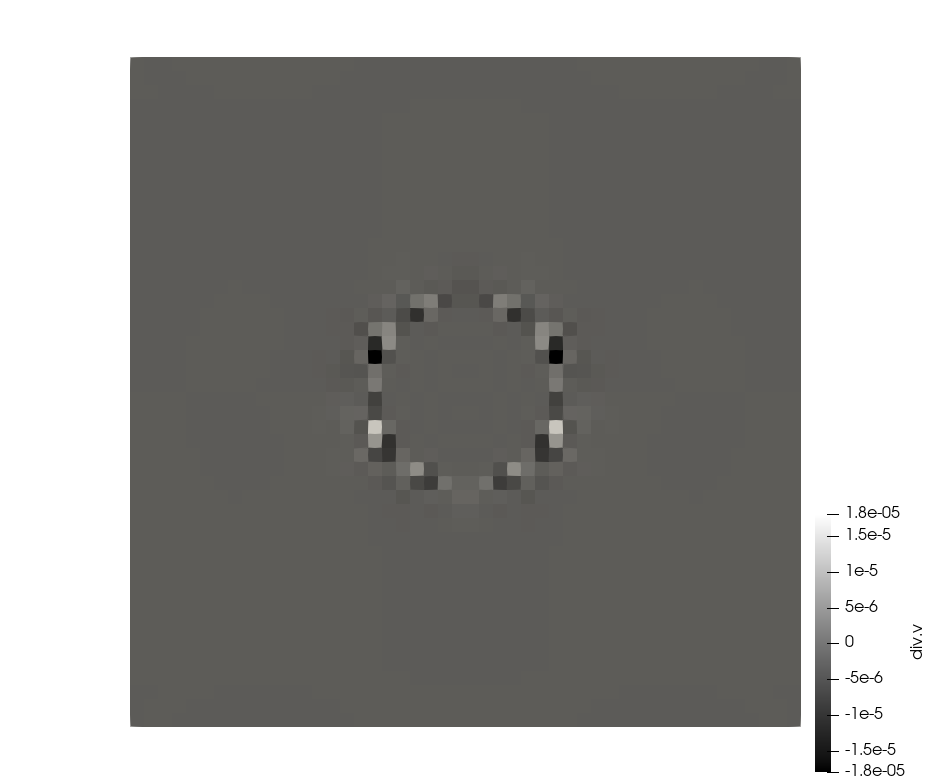
\includegraphics[width=5.7cm]{python_codes/fieldstone_111/results/n3_k5/divv}\\
{\captionfont Various fields for $n=3$ and $k=5$. Just because it is pretty.}
\end{center}


